\begin{frame}{Fitting for separation of $d(K^-, n)"\pi^{\pm}\Sigma^{\mp}"$}
  \small
  \begin{tabular}{cc}
    \begin{minipage}{0.7\hsize}
      \begin{enumerate}
      \item $K^- d \rightarrow K^0 "n" n_{detected}$\\
        $\rightarrow$ These events include 1-step \& 2-step 
      \item $K^- d \rightarrow "n" \pi^{\mp} \Sigma^{\pm}_{forward}$  $\Sigma^{\pm}_{forward} \rightarrow \pi^{\pm} n_{detected}$\\
        $\rightarrow$ Strangeness gives forward scattering baryon\\
        \hspace{3mm} Negligibly small in $K^0$ and $\Sigma_{forward}$ rejected events
      \item $K^- d \rightarrow \pi^{\mp} "\Sigma^{\pm}" n_{detected}$\\
        Recoiled $\bar{K}$ reacts with residual nucleon.\\
        Strangeness gives backward particles.
      \end{enumerate}
    \end{minipage}
    \begin{minipage}{0.3\hsize}
      \begin{figure}
        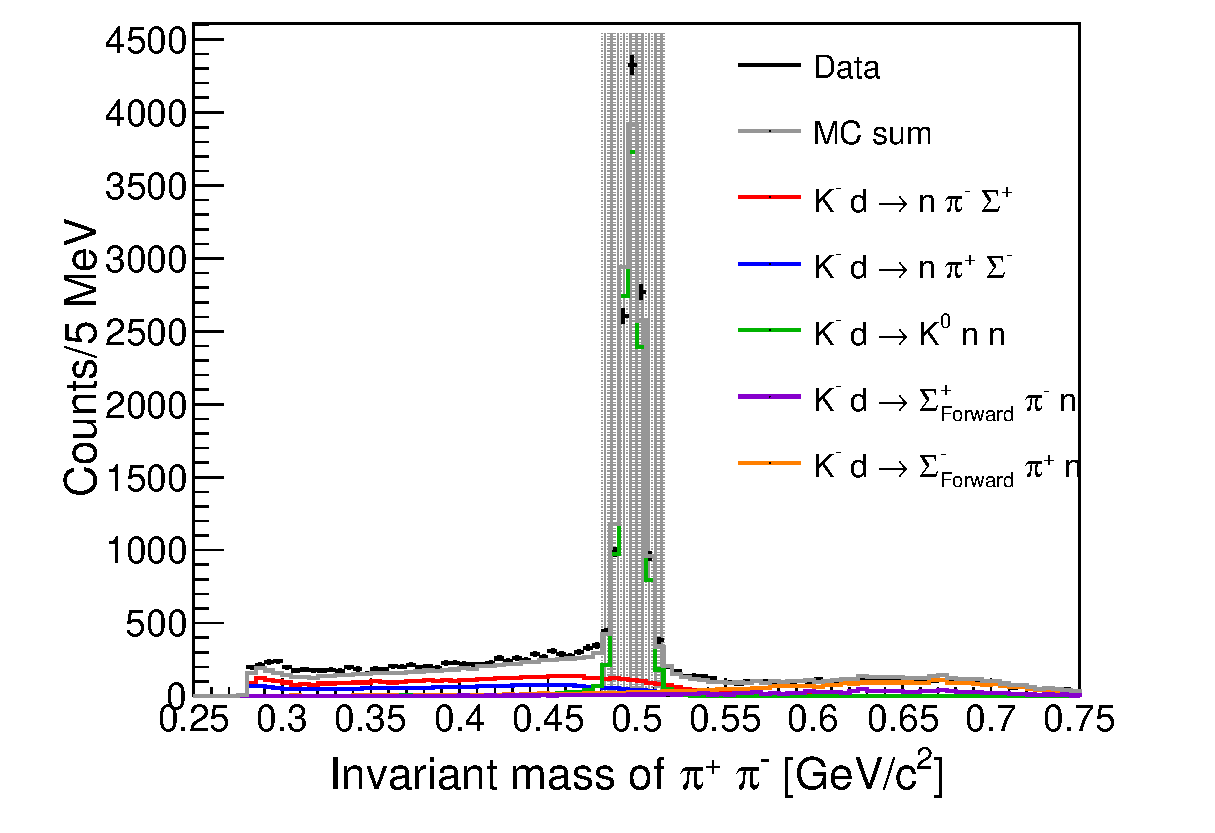
\includegraphics[width=2.5cm]{../pic/Run78/KN_ana/IM_pipi.eps}
        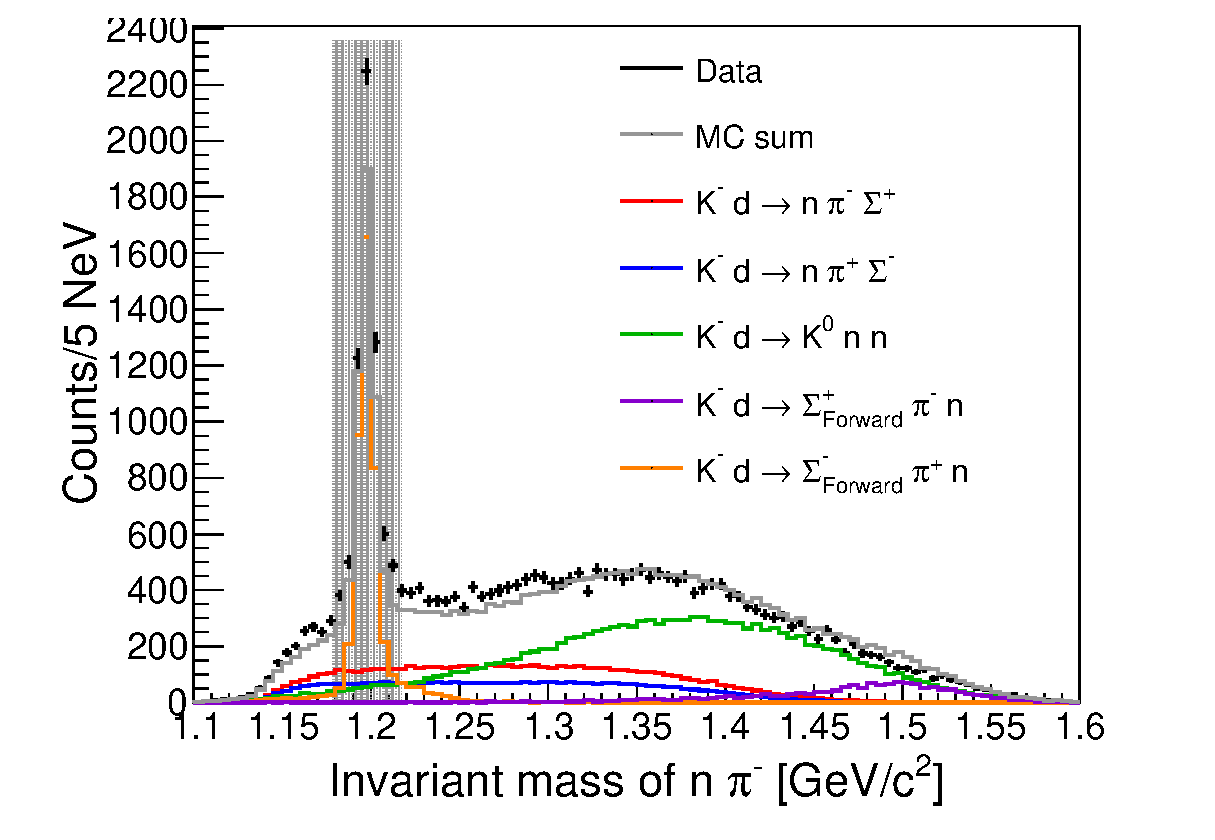
\includegraphics[width=2.5cm]{../pic/Run78/KN_ana/IM_npim.eps}
        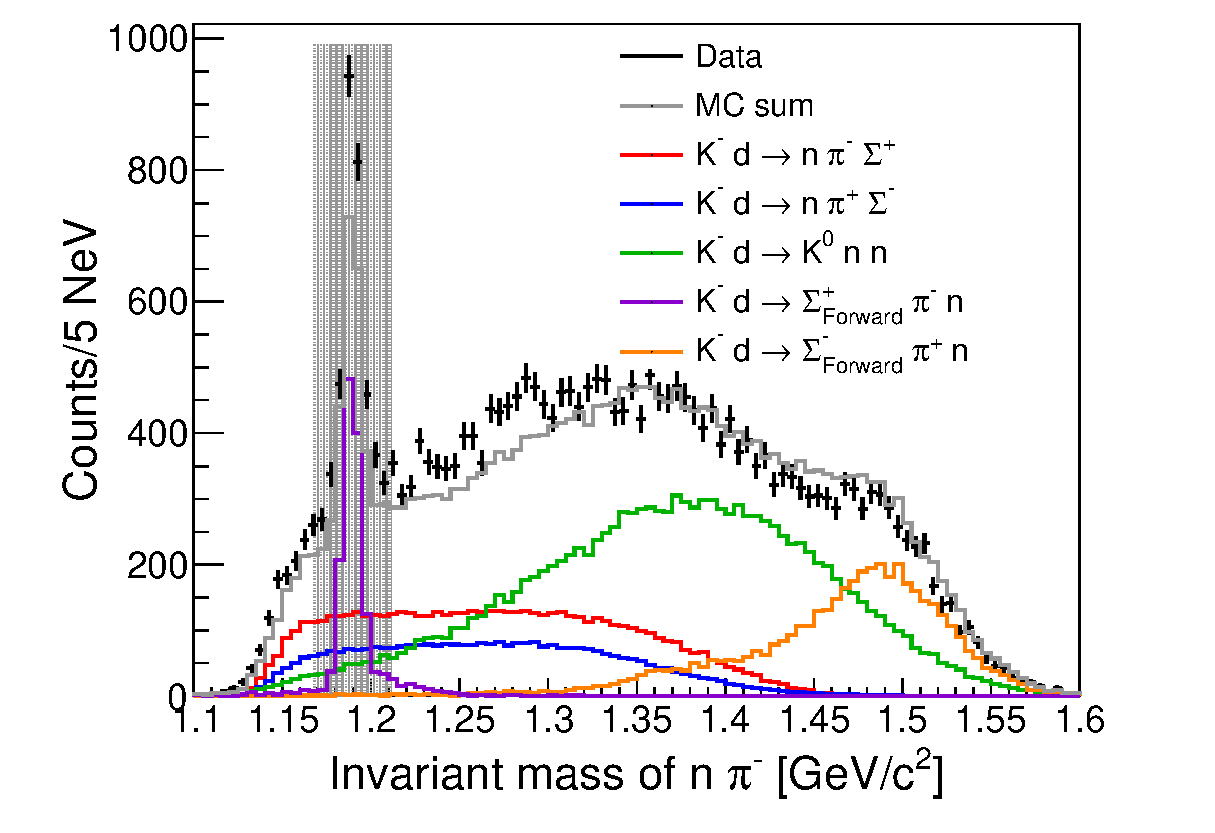
\includegraphics[width=2.5cm]{../pic/Run78/KN_ana/IM_npip.eps}
      \end{figure}
    \end{minipage}
  \end{tabular}

  \begin{tabular}{ccc}
    \begin{minipage}{0.2\hsize}
      \begin{figure}
        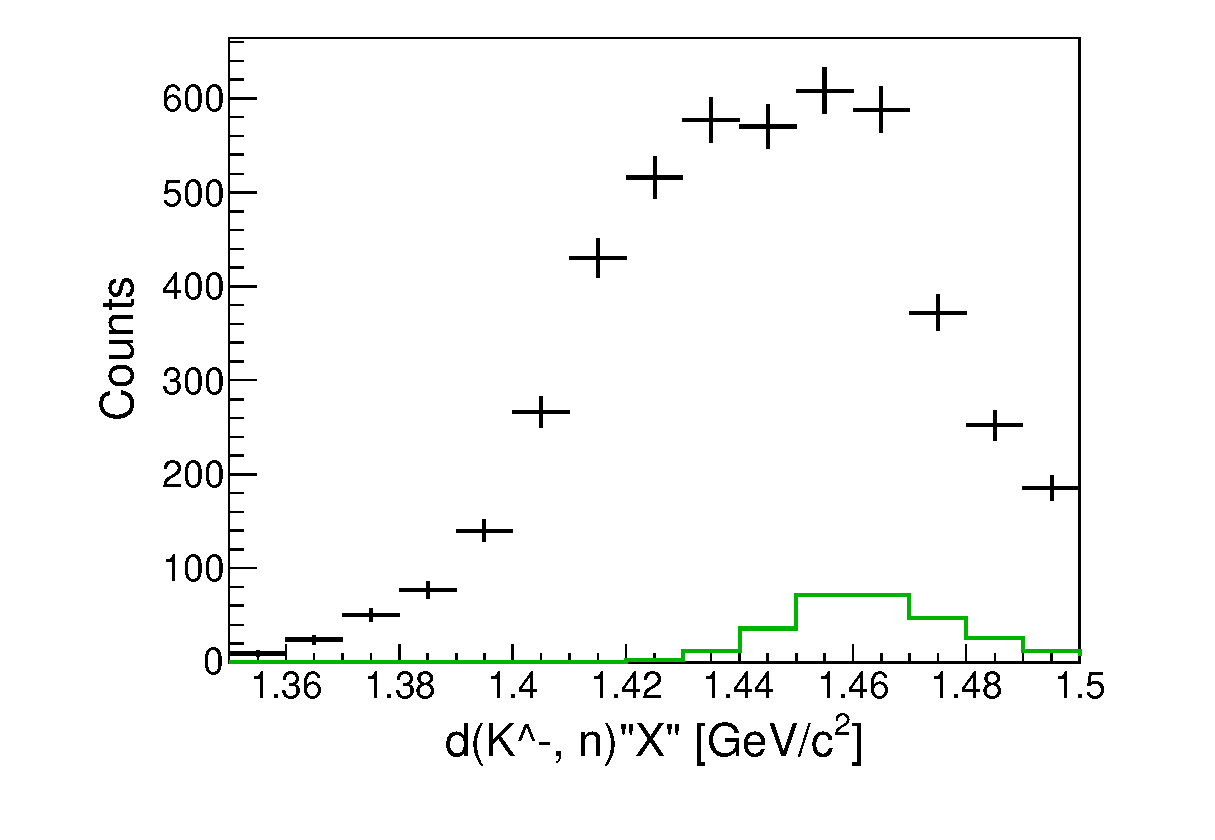
\includegraphics[width=2.5cm]{../pic/Run78//KN_ana_NC170_2sigma//KN_MM_woAll.eps}
      \end{figure}
    \end{minipage}
    \begin{minipage}{0.43\hsize}
      \scriptsize
      Left figure indicates $d(K^-, n)"\pi^{\mp}\Sigma^{\pm}"$,\\ which was rejected $K^0$ and $\Sigma^{\pm}_{forward}$
      \vspace{2mm}\\
      
      Right figure shows $d(K^-, n \pi^{\mp})"\Sigma^{\pm}"$ fitting. Above figure $\Sigma^+$ peak clearly seen.\\
      $\Sigma^-$ peak seen in right projection.
    \end{minipage}
    
    
    \begin{minipage}{0.3\hsize}
      \begin{figure}
        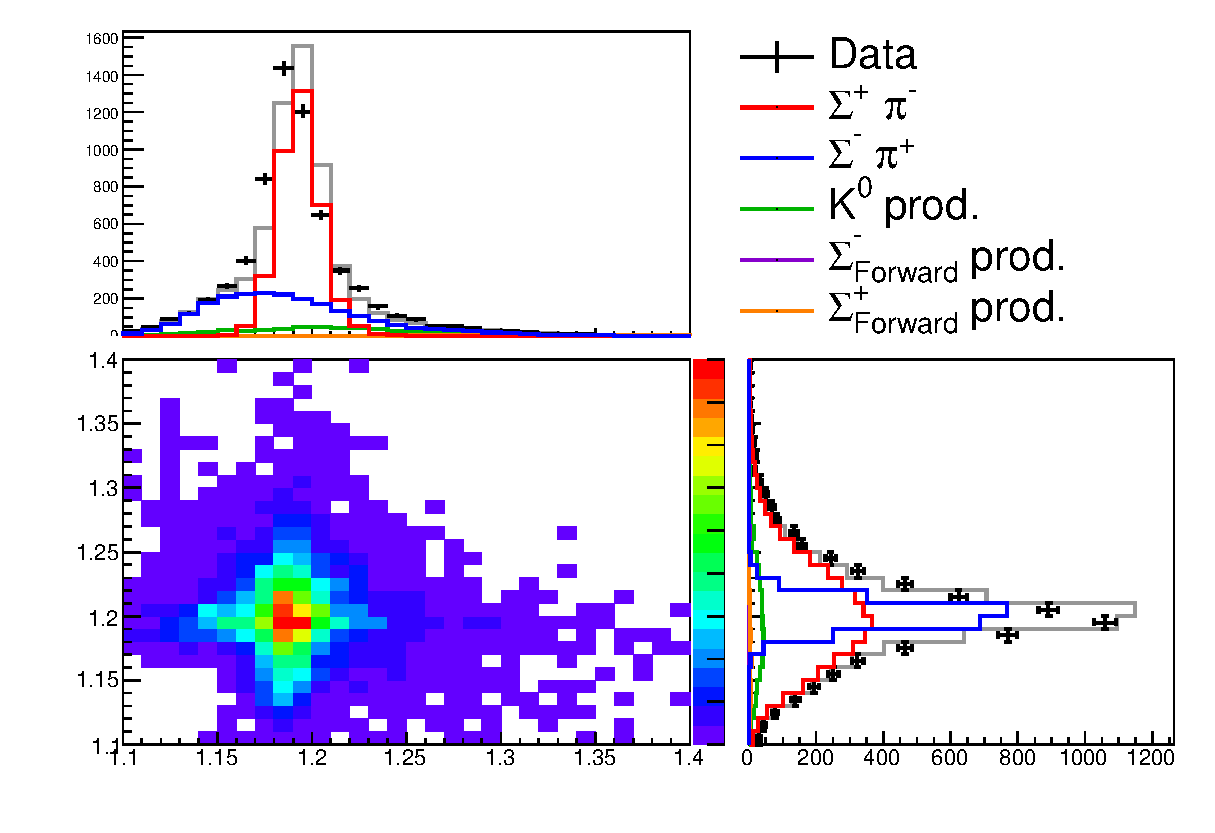
\includegraphics[width=4cm]{../pic/Run78//KN_ana_NC170_2sigma//KNpim_KNpip_MM.eps}
      \end{figure}
    \end{minipage}
  \end{tabular}
  
\end{frame}
